\documentclass{article}
\usepackage{graphicx}
\usepackage{amsmath}
\usepackage{amsfonts}
\usepackage{amssymb}
\usepackage{listings}
\begin{document}

See discussions, stats, and author profiles for this publication at: https://www.researchgate.net/publication/282352778

\section{Comparative study of van der Waals corrections to the bulk properties of graphite}

\textbf{Article} in Journal of Physics: Condensed Matter · September 2015 DOI: 10.1088/0953-8984/27/41/415502



\includegraphics{_page_0_Picture_4.png}


All content following this page was uploaded by Celso Ricardo Rêgo on 17 March 2016.



\includegraphics{_page_1_Picture_0.png}


Home Search Collections Journals About Contact us My IOPscience

Comparative study of van der Waals corrections to the bulk properties of graphite

This content has been downloaded from IOPscience. Please scroll down to see the full text. View the table of contents for this issue, or go to the journal homepage for more 2015 J. Phys.: Condens. Matter 27 415502 (http://iopscience.iop.org/0953-8984/27/41/415502)

Download details:

IP Address: 141.223.163.109 This content was downloaded on 04/03/2016 at 23:01

Please note that terms and conditions apply.

J. Phys.: Condens. Matter 27 (2015) 415502 (10pp) doi:10.1088/0953-8984/27/41/415502

\section{\textbf{Comparative study of van der Waals corrections to the bulk properties of graphite}}

\section{\textbf{Celso R C Rêgo}1,2**, Luiz N Oliveira\textbf{1}, Polina Tereshchuk**3 \textbf{and Juarez L F Da Silva}3}

1 São Carlos Institute of Physics, University of São Paulo, PO Box 369, 13560-970, São Carlos, SP, Brazil

2 Amazonas State University, Av. Djalma Batista 3578, Flores, 69050-010, Manaus, AM, Brazil

3 São Carlos Institute of Chemistry, University of São Paulo, PO Box 780, 13560-970, São Carlos, SP, Brazil

E-mail: juarez\_dasilva@iqsc.usp.br

Received 15 June 2015, revised 15 August 2015 Accepted for publication 14 September 2015 Published 29 September 2015



\includegraphics{_page_2_Picture_10.png}


\section{\textbf{Abstract}}

C R C Rêgo \textit{et al}

© 2015 IOP Publishing Ltd

J. Phys.: Condens. Matter

Journal of Physics: Condensed Matter

415502

JCOMEL

2015

27

IOP

Printed in the UK

10.1088/0953-8984/27/41/415502

CM

0953-8984

41

\textbf{Papers}

Comparative study of van der Waals corrections to the bulk properties of graphite

Graphite is a stack of honeycomb (graphene) layers bound together by nonlocal, long-range van der Waals (vdW) forces, which are poorly described by density functional theory (DFT) within local or semilocal exchange-correlation functionals. Several approximations have been proposed to add a vdW correction to the DFT total energies (Stefan Grimme (D2 and D3) with different damping functions (D3-BJ), Tkatchenko–Scheffler (TS) without and with self-consistent screening (TS + SCS) effects). Those corrections have remarkly improved the agreement between our results and experiment for the interlayer distance (from 3.8 to 0.1\%) and high-level random-phase approximation (RPA) calculations for interlayer binding energy (from 56.2 to 0.6\%). We report a systematic investigation of various structural, energetic and electron properties with the aforementioned vdW corrections followed by comparison with experimental and theoretical RPA data. Comparison between the resulting relative errors shows that the TS + SCS correction provides the best results; the other corrections yield significantly larger errors for at least one of the studied properties. If considerations of computational costs or convergence problems rule out the TS + SCS approach, we recommend the D3-BJ correction. Comparison between the computed πzΓ-splitting and experimental results shows disagreements of 10\% or more with all vdW corrections. Even the computationally more expensive hybrid PBE0 has proved unable to improve the agreement with the measured splitting. Our results indicate that improvements of the exchangecorrelation functionals beyond the vdW corrections are necessary to accurately describe the band structure of graphite.

Keywords: density functional theory, graphite, van der Waals corrections

(Some figures may appear in colour only in the online journal)

\section{I. \textbf{Introduction}}

The technological importance of carbon materials such as graphite, fullerenes, nanotubes, and graphene has steadily grown in the last decades [1, 2] due to the wide range of applications, which includes solid lubricant, energy storage, adsorbents, batteries, microelectronics, biomedicine, etc [3–6]. The resulting reseach on supported graphene layers on metals and semiconductor surfaces has revived interest in the weak interaction between carbon monolayers and solid surfaces, as well as in weak interactions within carbon compounds [5, 7, 8]. Among carbon materials, graphite is special due to the presence of covalent (in plane) and weak van der Waals (vdW) interactions between the graphene layers with honeycomb symmetry and has hence been widely employed as a testbed for theoretical developments.

The stacking of the honeycomb layers in graphite can occur in two forms, namely, AB (hexagonal), which is more common, and ABC (rhombohedral) [9–11]. To focus our discussion, we have chosen the former, known as the Bernal structure, which contains four carbon atoms in the primitive unit cell with space group P63/mmc. On the experimental front, our understanding of the nature and strength of the graphitic interlayer binding is limited. Not even the spatial dependence of the interlayer interaction has been firmly determined, an uncertainty that raises doubts concerning the vdW interactions in graphitic systems [12, 13]. Indirect measurements have yielded various results (for AB stacking), namely, from −31(2) to −52(5) meV/atom [14–17], which has motivated a large number of studies aiming to obtain an accurate theoretical estimate for the interlayer binding energy.

It has long been known that the intralayer chemical binding in graphite is much stronger than the interlayer vdW interaction [14–16]. The short bond lenghts resulting from the intralayer binding are well described by density-function theory (DFT) [18, 19] in the Perdew–Burke–Erzerhof (PBE) [20] generalized-gradient approximation (GGA) [21] for the exchange-correlation (XC) functional. The binding between layers is governed by nonlocal long-range dispersion forces [14], which are poorly described by DFT within local [22] or semilocal XC functionals [23, 24]. \textit{Ab initio} calculations using multireference configuration interaction with a doublezeta plus polarization basis set have yielded 1.36eV per C atom as the correlation-energy contribution to the cohesive energy of a graphite layer [25]. Alternative numerical procedures have also been employed, such as the quantum Monte Carlo (QMC) [26, 27] method and random-phase approximation (RPA) [28, 29].

For example, QMC calculations by Spanu \textit{et al} [30] have yielded Eb = −56 meV/atom for graphite AB, close to the experimental value reported by Zacharia \textit{et al} (52 meV/atom) [16]. RPA-based methods can be combined with DFT computations to exploit the translational symmetry of the system. A good example is the study by Lèbegue \textit{et al} [29], which found Eb = −48 meV/atom and comparably accurate elastic constants. Unfortunately, both QMC and RPA calculations require enormous computational efforts, which limits the range of applications. Few periodic layered materials are within the reach of either method.

To overcome these problems, different GGA functionals combined with nonlocal correlations or direct functionals for the vdW nonlocal correlation [31–34] have recently been proposed. The resulting binding energies for graphite [33, 34] are significantly improved with respect to the binding energies from PBE or hybrid meta-GGA calculations, which are too small to satisfy stability requirements [31–33]. To date, several corrections to plain DFT have been proposed to accurately describe the vdW corrections at lower computational cost, namely the Tkatchenko–Scheffler (TS) correction without [35] and with [36] self-consistent screening (TS + SCS), and C R C Rêgo \textit{et al}

the D2 and D3 corrections put forward by Grimme [32, 37]. Gobre and Tkatchenko employed the TS and TS + SCS corrections, as implemented in the Fritz-Haber Institute \textit{ab initio} molecular simulation (FHI-aims) package [38], to study vdW interactions in single- and multilayer graphene, fullerenes, single-wall carbon nanotubes and graphene nanoribbons [7]. They found that the TS + SCS correction yields good results for the interlayer binding energies and reliably describes raregas solids, the acid test of vdW corrections.

In a parallel study, Grimme \textit{et al} considered numerous systems and found that the D3 correction constitutes an improvement over D2, for layered materials in particular [32]. Recently, Bucko \textit{et al} applied the TS, TS + SCS, and D2 corrections to the PBE functional, as implemented in the Vienna \textit{ab initio} Simulation Package (VASP) [39, 40], to study a wide range of systems, including layered materials [41], molecular solids [42], and ionic surfaces [43]. For graphite, the target of the present work, Bucko \textit{et al} [41], Grimme et al [32], and Gobre and Tkatchenko [7] focused on the interlayer binding energy and bulk modulus. Finer details, such as the curvature of the interlayer binding energy and the splitting between levels in the band structure, were not discussed in those studies, even though they impose demanding checks on the accuracy resulting from vdW corrections. Furthermore, the D3 correction and its variants with different damping functions have not been applied to graphite.

To investigate the performance of vdW corrections (TS, TS + SCS, D2, D3) to plain DFT in computations of the bulk properties of graphite, we have calculated such structural and energetic properties of graphite as lattice parameters, the bulk modulus, cohesive energy, interlayer binding energy and curvature of the interlayer binding energy. In addition, we have given special attention to a feature of the computed band structures, the πz-splitting at the Γ-point. Our results and analysis indicate that the TS + SCS correction is the preferred method for the vdW corrections. In case that convergence or computational cost be a problem, we recommend the D3-BJ correction.

\subsubsection{II. \textbf{Theoretical approach and computational details}}

Our total-energy DFT calculations rely on the PBE XC functional. To accurately describe the interlayer distance in graphite, we have added vdW corrections to the dispersion forces, the vdW-corrected DFT total energy Etot being obtained as follows:

$$E_{\rm tot}=E_{\rm tot}^{\rm DFT}+E_{\rm tot}^{\rm wdW},\tag{1}$$

where Etot DFT is the DFT-PBE total energy, and Etot vdW is the correction to the total energy due to the vdW interactions, which is given by the following equation:

$E_{\rm tot}^{\rm vdW}=E^{(2)}+E^{(3)}$.

The first term on the right-hand side of equation (2) stems from the dipole–dipole interaction induced by quantum fluctuations in the electron density, while E(3) comes from the triple dipole dispersion term found in the third-order perturbation treatment of three atoms ijk [32, 44]. Within this framework, the accuracy depends on the dispersion coefficients CAB 6 , which determines E(2), and/or \textit{CABC} 9 , which determines E(3), where A, B, and C indicates the chemical species. The two coefficients can be extracted from experimental data, or they can be computed, a number of theoretical approaches having been proposed. Of special interest here are the TS, TS + SCS, D2, and D3 corrections as implemented in VASP, upon which our computations are based.

Since the dipolar interactions diverge as the separation R → 0, the corrections E(2) and E(3) include a multiplicative factor f R( ) , , R s, d damp 0 , a function of R defined by three parameters: R0, s, and d. More specifically, f R( ) , , R s, d damp 0 vanishes (approaches unity) at very small (large) distances, and the transition from f R damp ( → 0 0 ) = to f R( → ∞ =) 1 damp is controlled by R0, s, and d [35, 41]. Roughly speaking, one expects the transition to occur at a distance scale set by the sum R0 of the vdW radii of the two interacting species. The scaling factor s, which depends on the employed exchangecorrelation functional only, defines more precisely the transition point: f R( ) , , R s, d damp 0 rises sharply from zero to unity around R = sR0 . Finally, the parameter d, also dependent on the XC functional only, defines the abruptness of the transition. Different ways to calculate the damping function have recently been proposed, among them a procedure defined within the Many-Body Dispersion (MBD) method [45]. To investigate the effect of the damping functions on the accuracy of the results, we probed a few expressions for f R( ) , , R s, d damp 0 , such as the zero and Becke–Johnson dampings implemented in the D3-correction approach, denoted D3 and D3-BJ, respectively.

In the D2 scheme [37],

$$E^{(2)}=-\frac{1}{2}\sum_{ij}\int_{\rm damp,2}\left(R_{ij}\right)\frac{C_{6}^{AB}}{R_{ij}^{6}},\tag{3}$$

while the second term on the right-hand side of equation (2), E(3), is zero. The CAB 6 coefficients are found from the equation

$$C_{6}^{AB}=\sqrt{C_{6}^{A}C_{6}^{B}}\,,\tag{4}$$

and

$\bf C_{6}^{A}=0.05NI_{p}^{A}\alpha^{A}$, (5)

where the atomic ionization potentials Ip and static dipole polarizabilities α were obtained from PBE0 [46] calculations with N =2, 10, 18, 36, and 54 for atoms in rows 1–5 of the periodic table.

In the D3 scheme [32], both terms on the right-hand side of equation (2) are nonzero, and

$$E^{(3)}=\gamma\sum_{ijk}f_{\rm damp,3}(R_{ijk})\frac{C_{9}^{ABC}}{(R_{ij}R_{jk}R_{kj})^{3}}.\tag{6}$$

Here, the constant γ depends on the internal angles of the triangle formed by Rij, Rjk and Rki [44], and the ternary coefficients \textit{CABC} 9 are obtained from the binary dispersion coefficients CAB 6 as follows. The binary coefficients are given

by the modified Casimir–Polder integral [47]:

$$C_{6}^{A B}=\frac{3}{\pi}\int_{0}^{\infty}\mathrm{d}\omega\frac{1}{m}\bigg{[}\alpha^{A_{m}H_{n}}(\mathrm{i}\omega)-\frac{n}{2}\alpha^{H_{2}}(\mathrm{i}\omega)\bigg{]}\tag{7}$$

$$\times\frac{1}{k}\bigg{[}\alpha^{B_{k}H_{0}}({\rm i}\omega)-\frac{l}{2}\alpha^{H_{0}}({\rm i}\omega)\bigg{]},\tag{8}$$

which takes the polarizabilities of simple molecules with well-defined electronic structures into account, instead of free-atom polarizabilities.

When the polarizabilities of the sample molecules are substituted on the right-hand side of equation (7), an interpolation procedure yields the chemically reasonable coordination numbers for the system under study and determines the dispersion coefficients. The ternary dispersion coefficients \textit{CABC} 9 are then obtained from the expression

$$C_{9}^{ABC}\approx-\sqrt{C_{6}^{AB}C_{6}^{AC}C_{6}^{BC}}.\tag{9}$$

In the TS and TS + SCS schemes, the analytical form for E(2) is almost the same as in the D2 and D3 schemes, while E(3) is null. To determine the dispersion coefficients CAA 6 , a different concept is exploited. In the TS approach, the parameters CAB 6 are obtained from the expression

$$C_{6}^{AB}=\frac{2C_{6}^{AA}C_{6}^{BB}}{\left(\frac{\alpha_{0}^{R}}{\alpha_{0}^{A}}C_{6}^{AA}+\frac{\alpha_{0}^{A}}{\alpha_{0}^{B}}C_{6}^{BB}\right)},\tag{10}$$

and the dispersion coefficients from the equality

$$C_{6}^{AA}=\left(\frac{V_{\rm eff}^{A}}{V_{\rm free}^{A}}\right)^{2}(C_{6}^{AA})^{\rm free},\tag{11}$$

where the ratio V /V A A eff free between the effective and free (noninteracting) atomic volumes are obtained from the Hirshfeld partitioning of the computed electronic densities for the interacting system and free atom, and α A 0 and α B 0 are the static polarizabilities [35].

The TS approach disregards the screening of the electrostatic interaction between distant dipoles, which has no effect upon the polarizabilities of free atoms. This approximation is less adequate to compute the polarizabilities of atoms in large molecules or condensed phases. To account for screening, the TS + SCS approach treats the environment as a dipole field [36], and substitutes a set of quantum harmonic-oscillator densities for the atomic densities, so that the spatial dependence can be integrated out. The solution of the resulting SCS equation determines the frequency-dependent screened polarizabilities α ω( ) i A SCS [36], where the homonuclear dispersion coefficients CAA 6 are computed from the Casimir–Polder formula [47]

$$C_{6}^{AA}=\frac{3}{\pi}\int_{0}^{\infty}\left(\alpha_{\rm scs}^{A}({\rm i}\omega)\right)^{2}{\rm d}\omega.\tag{12}$$

An improved version of the TS method recently developed by Tkatchenko \textit{et al} includes electrodynamic response (TS + SCS) and many-body (TS + MBD) effects [45]. The latter has been proven equivalent to an RPA computation of dispersion energies [48]; both methods yield accurate results for the interlayer binding energy of graphite. Moreover, other methods have been recently proposed to include vdW interactions in DFT, e.g. the vdW-Quantum Harmonic Oscillator-Wannier function method [49], which properly describes the adsorption of molecules on graphene. Additional details on the D2, D3, TS, and TS + SCS vdW corrections can be found elsewhere [7, 32, 35–37, 41–43, 50].

We have solved the Kohn–Sham equations with the allelectron projected augmented wave (PAW) method [51, 52], as implemented in VASP [40], which uses plane waves under periodic boundary conditions as its basis set. We have considered the PAW projectors, as provided within VASP [52], employing the 2s p22 2 carbon valence electrons. To obtain the equilibrium volumes, we have calculated the stress tensor and minimized the stress and atomic forces. Given the small magnitude of the interlayer binding energies and strong dependence of the stress tensor on the number of plane waves, we have systematically studied the equilibrium volume as a function of the cutoff energy and number of k-points in the Brillouin-zone.

We have found that a cutoff energy of 900eV is sufficient to guarantee convergence, deviations smaller than 0.002\% resulting from comparing the results with those of a 1050eV cutoff computation. The converged results with k-meshes of 21 2 × ×1 7 and 42 4 × ×2 14 points were found to differ by 0.05\%. For the total-energy calculations, we have employed a cutoff energy of 450 eV. For all calculations, the search for the equilibrium volume was interrupted once the forces were smaller than 0.010eV − A˚ 1 , with a total-energy convergence of 10−6 eV.

\section{\textbf{III. Results and discussion}}

To compare the performance of different vdW corrections, we have calculated the lattice parameters, bulk modulus, cohesive energy, interlayer binding energy, curvature of the interlayer binding energy (second and third derivatives), and band structure of graphite. The most important results are summarized in Table 1 along with theoretical and experimental findings. We have only included previous theoretical studies for which the graphite properties were calculated at the equilibrium lattice constants optimized by total energy calculations. As benchmarks, we have chosen the precise experimental data for the equilibrium geometry and cohesive energy [53–57], except for the interlayer binding energy, for which we use the theoretical, high-level RPA results [29].

\subsubsection{\textit{III.A. Equilibrium lattice parameters}}

Table 1 lists the equilibrium lattice parameters a0 (on the graphite plane) and c0 (perpendicular to the graphite plane), compared with experimental and previous theoretical results. As expected, the PBE estimate for a0 is accurate, only 0.16\% above the experimental value. As also expected, given the attractive nature of the interactions, the vdW corrections reduce a0. In particular, the D2, D3, D3-BJ, and TS + SCS vdW corrections bring a0 into closer agreement with the experimental result: the relative error ranges from −0.04 to +0.08\%. By contrast, the absolute value of the −0.16\% relative deviation resulting from the TS computation equals that of the PBE computation.

To compute c0, we have fitted the c-dependent binding energies to Chebyshev polynomials and identified the separation at which the first derivative equals zero, as detailed in appendix A. As reported in previous studies [29, 30, 32, 41, 42], the PBE functional yields a result 25.5\% larger than the experimental value, a deviation commonly attributed to the absence of non-local long-range correlations in the PBE functional. The local density approximation (LDA) yields c = 6.57 A˚ 0 , which underestimates the lattice parameter by 2\% [22]. The vdW corrections provide substantial improvement over the PBE estimate. The resulting relative errors are −3.9\% (D2),+3.9\% (D3),+0.1\% (D3-BJ),−0.2\% (TS), and −1.7\% (TS + SCS). Only the D3-BJ, TS, and TS + SCS corrections yield a0 and c0 estimates under the 2.0\% relativeerror limit, typical of local- and semilocal-functional computations for metals and semiconductors [58].

\subsubsection{\textit{III.B. Cohesive energy}}

From the equilibrium total energy and C free-atom total energy, we have calculated the graphite cohesive energy. PBE yields −7.85 eV/atom,+6.5\% larger than the experimental value (−7.37 eV/atom [57, 61]), a result whose accuracy is comparable to that of PBE cohesive-energy computations for metals and semiconductors [62–64]. Our estimate deviates from previous DFT results,−7.55 eV/ atom [65], and −7.34 eV/atom [66]. Part of the error is due to the standard PAW C projector in our computation, which yields less accurate total energies than the hard PAW C projectors, i.e. about 0.10 eV/atom. The chief contribution to the error in the calculated cohesive energy nonetheless comes from overbinding in the intralayer interactions, a shortcoming of the PBE calculations that the vdW corrections cannot remedy. In fact, given their attractive contribution to the total energy, all the vdW corrections magnify the relative error in the cohesive energy. With the D3-BJ correction, for instance, the relative error grows from +6.5 to +8.4\%.

\subsubsection{\textit{III.C. Interlayer binding energy}}

One of the key energetic properties of graphite is the binding energy between the honeycomb layers, i.e. the interlayer binding energy [33, 41, 59], which differs from the exfoliation energy [14] (i.e. the energy required to remove one graphite sheet from a semi-infinite film), or the interaction energy of

\textbf{Table 1.} Bulk properties of graphite: equilibrium lattice parameters a0 and c0, bulk modulus B0, bulk modulus first derivative B′, curvature C33 and curvature derivative C333 of the interlayer binding energy, cohesive energy Ecoh, and interlayer binding energy Eb computed with distinct dispersion corrections.

|                      ||        ||        ||            ||       ||           ||             || −Ecoh      || −Eb         ||             |
| ---                  || ---    || ---    || ---        || ---   || ---       || ---         || ---        || ---         || ---         |
| Procedure            || a0 (Å) || c0 (Å) || B0 (GPa)   || B′ 0  || C33 (GPa) || −C333 (GPa) || (eV/ atom) || (meV/ atom) || References  |
| PBE                  || 2.466  || 8.755  || 1.6        || 15.70 || 0.55      || 4           || 7.85       || 1.2         || This work   |
| PBE + D2             || 2.461  || 6.444  || 40.2       || 13.02 || 22.04     || 178         || 7.96       || 55.04       || This work   |
| PBE + D3             || 2.464  || 6.965  || 23.8       || 4.81  || 13.09     || 90          || 7.93       || 47.30       || This work   |
| PBE + D3-BJ          || 2.464  || 6.745  || 30.1       || 10.13 || 17.16     || 115         || 7.99       || 52.36       || This work   |
| PBE + TS             || 2.458  || 6.665  || 56.1       || 10.05 || 34.61     || 188         || 7.98       || 81.34       || This work   |
| PBE + TS + SCS       || 2.461  || 6.633  || 40.5       || 12.77 || 26.79     || 184         || 7.97       || 53.76       || This work   |
| RPA                  || 2.46   || 6.68   ||            ||       || 36        ||             ||            || 48          || [29]        |
| ACFD-RPA             || 2.46   || 6.68   ||            ||       ||           || 530         ||            ||             || [56]        |
| QMC                  || 2.46   || 6.852  ||            ||       ||           ||             ||            || 56          || [30]        |
| LDA                  || 2.46   || 6.66   ||            ||       || 29.5      ||             ||            || 24          || [29]        |
| LDA                  || 2.46   || 6.75   ||            ||       || 29.9      ||             ||            || 9.432       || [33]        |
| PBE                  || 2.46   || 7.809  ||            ||       || 1.2       ||             ||            || 0.399       || [33]        |
| PBE                  || 2.47   || 8.84   || 1          ||       ||           ||             || 7.99       ||             || [42]        |
| PBE                  || 2.466  || 9.62   || 0.8        ||       ||           ||             ||            || 0.6         || [31]        |
| revB86B              || 2.47   || 6.72   ||            ||       ||           ||             ||            || 21.0        || [34]        |
| C09 (vdw)            || 2.47   || 6.54   ||            ||       ||           ||             ||            || 26.9        || [34]        |
| cx13 (vdw)           || 2.47   || 6.65   ||            ||       ||           ||             ||            || 23.0        || [34]        |
| optPBE (vdW)         || 2.47   || 6.98   ||            ||       ||           ||             ||            || 22.7        || [34]        |
| optB88 (vdW)         || 2.47   || 6.76   ||            ||       ||           ||             ||            || 25.1        || [34]        |
| optB86B(vdW)         || 2.47   || 6.72   ||            ||       ||           ||             ||            || 24.8        || [34]        |
| vdW-DF               || 2.47   || 7.52   || 12         ||       || 13        ||             ||            || 24          || [59]        |
| DF1                  || 2.46   || 7.199  ||            ||       || 23.0      ||             ||            || 18.90       || [33]        |
| DF2                  || 2.46   || 6.944  ||            ||       || 33.5      ||             ||            || 18.63       || [33]        |
| DF1(PBE)             || 2.46   || 6.892  ||            ||       || 35.6      ||             ||            || 25.67       || [33]        |
| VV10                 || 2.46   || 6.777  ||            ||       || 46.1      ||             ||            || 27.07       || [33]        |
| PBE + D2             || 2.46   || 6.740  ||            ||       || 44.0      ||             ||            || 21.15       || [33]        |
| PBE + D2             || 2.46   || 6.45   || 38         ||       ||           ||             || 8.10       ||             || [42]        |
| PBE + D2             || 2.466  || 6.43   || 46.5       ||       ||           ||             ||            || 54.1        || [31]        |
| PBE + TS             || 2.46   || 6.68   || 59         ||       ||           ||             ||            || 82          || [41]        |
| PBE + TS             || 2.46   || 6.604  ||            ||       ||           ||             ||            || 87.83       || [7]         |
| PBE + TS + SCS       || 2.46   || 6.604  ||            ||       ||           ||             ||            || 50.54       || [7]         |
| PBE + TS + SCS       || 2.46   || 6.75   || 43         ||       ||           ||             ||            || 55          || [41]        |
| PBE + TS + SCS + MBD || 2.46   || 6.70   ||            ||       ||           ||             ||            || 48          || [45]        |
| Experiment           || 2.46   ||        ||            ||       ||           ||             ||            || 52 5 ±      || [16]        |
| Experiment           || 2.462  || 6.707  || 35.8 ± 1.6 ||       ||           ||             ||            ||             || [53]        |
| Experiment           || 2.463  || 6.712  ||            ||       || 38.7      ||             ||            ||             || [55]        |
| Experiment           ||        ||        ||            ||       ||           ||             ||            || 31 2 ±      || [17]        |
| Experiment           || 2.46   || 6.70   ||            ||       ||           ||             ||            || 35          || [15]        |
| Experiment           ||        ||        ||            ||       ||           ||             ||            || 42.64       || [14]        |
| Experiment           || 2.603  || 6.706  || 33.8       || 8.9   ||           ||             ||            ||             || [54]        |
| Experiment           ||        ||        ||            ||       ||           ||             || 7.37       ||             || [57]        |
| Experiment           ||        ||        ||            ||       || 36.5      ||             ||            ||             || [60]        |
| Reference datum      || 2.462  || 6.707  || 35.6       || 8.9   || 37.6      || 530         || 7.37       || 48          || [29, 53–57] |

\textit{Note}: For comparison, the last row lists the average experimental results and the only available theoretical estimate for C333.

two graphene sheets [32]. Accordingly, we have computed the interlayer binding energy per atom Eb as a function of the interlayer separation (c/2) at fixed a = 2.466 A˚ . The interlayer binding energy is defined by the equation

$$E_{\rm b}(c)=-\frac{E_{\rm tot}(c)-E_{\rm tot}(c=\infty)}{4},\tag{13}$$

where Etot( ) c is the total energy.

We have computed the right-hand side of equation (13) in the interval cexp e /2 ⩽ ⩽c c3 xp, with 3c = 20.1 A˚ exp substituted for c = ∞. Figure 2 shows the resulting interlayer binding energies for the vdW corrections under study, compared to the experimental data. For visual convenience, the RPA binding energies [29] (blue open circles) are shown in the inset, compared with the PBE + TS + SCS (black open diamonds) and experimental binding energies (cyan open circles).


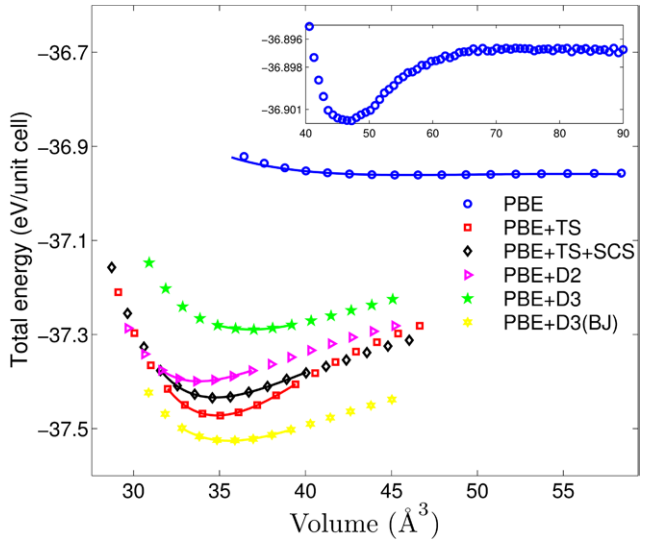
\includegraphics{_page_7_Figure_1.png}


\textbf{Figure 1.} Total energy per unit cell (four atoms) as a function of volume, for graphite. The blue open circles, red open squares, black open diamonds, magenta open triangles, green solid stars, and yellow solid hexagons represent the PBE, PBE + TS, PBE + TS + SCS, D2, D3 and D3-BJ calculations, respectively. Near each minimum, a solid line fits equation (14) to the computed energies. The expanded vertical scale in the inset brings out the shallow minimum of the PBE curve.

Table 1 compares the binding energy at the equilibrium distance c0 for each computational approach with the experimental data, which spread from −31(2) to −52(5) meV/atom [14–17]. The RPA [29] and QMC [30] results are closer to the upper limit,−52(5) meV/atom. The D2, D3, D3-BJ, TS, and TS + SCS corrections overestimate the reference binding energy (−48 meV/atom by 14.7\%, 1.45\%, 9.08\%, 69.45\%, and 12.01\%, respectively. Thus, except for the TS method, the vdW corrections yield great improvement over the PBE functional (1.2 meV/atom). Comparison with the high-level RPA results and with the experimental data shows that the D3 correction yields the smallest error.

\subsubsection{\textit{III.D. Bulk modulus and its first derivative}}

Another ground-state property affording comparison with experimental data is the equilibrium curvature of the total energy as a function of volume, i.e. the bulk modulus B0 and its first derivative B′ 0. To compute the volume dependence of the total energy, we have considered a set of equally spaced volumes, for each of which a and c were optimized. To calculate B0 and B′ 0, we have fitted the symbols representing the calculated total energies in figure 1 with the Birch–Murnaghan equation of state (solid lines) [67],

$$E_{\rm tot}(V)=E_{0}+\frac{9V_{0}B_{0}}{16}\{\gamma^{3}B_{0}^{\prime}-\gamma^{2}[4\gamma-2]\},\tag{14}$$

where γ = − ( ) V V0/ 1 2/3 , B B ′ 0 = ∂( ) /∂P V0, and V0 indicates the equilibrium volume. Table 1 lists the resulting B0 and B′ 0. The experimental B0 spread from 33.8 to 37.4 GPa [53–55, 68] (average 35.6 GPa), while the only available experimental datum for B′ 0 is 8.9 [54].

C R C Rêgo \textit{et al}

The PBE computation yields B0 = 1.6 GPa, far below the experimental range obtained from room-temperature measurements. Inspection of the blue open circles in figure 1 traces the poor agreement back to the unreasonable flatness of the potential-energy surface resulting from the PBE computation. The vdW corrections clearly improve the results, but the agreement is imperfect. The D3 (B0 = 23.8 GPa,−33.2\% deviation), and D3-BJ (B0 = 30.1 GPa,−15.5\% deviation) results underestimate the average experimental bulk modulus, while the D2 (B0 = 40.2 GPa,+12.9\% deviation), TS (B0 = 56.1 GPa,+57.6\% deviation), and TS + SCS (B0 = 40.5 GPa,+13.8\% deviation) results overestimate it. The PBE + D3-BJ, PBE + D2 and PBE + TS + SCS functionals yield bulk moduli in best agreement with the average experimental value.

In comparison with the experimental datum, the PBE + D3 correction underestimates B′ 0, while the other functionals overestimate it. The PBE estimate, B′ 0 = 15.7, overshoots the experimental value by 76.4\%. Here the vdW corrections also improve the agreement, but the results are still far from the experimental value: D3 yields B′ 0 = 4.8, 46.0\% below, D2 yields B′ 0 = 13.0, 46.0\% above, D3-BJ yields B′ 0 = 10.1, 13.5\% below , PBE + TS yields B′ 0 = 10.0, 12.4\% above, and PBE + TS + SCS yields B′ 0 = 12.7,−42.7\% above the measured derivative. The PBE + D3-BJ and PBE + TS functionals yield the B′ 0 value in best agreement with the experiment.

\subsubsection{\textit{III.E. Curvature of the interlayer binding energy}}

We now try to identify the source of the discrepancies between the calculated bulk moduli and the experimental data. To this end, we recall that the bulk modulus is related to elastic constants C\textit{11,} C12, C13, and C33 by the following equation [69]:

$$B_{0}=\frac{C_{33}(C_{11}+C_{12})-2C_{13}^{2}}{(C_{11}+C_{12})+2C_{33}-4C_{13}}.\tag{15}$$

We will here focus our discussion on the second and third order elastic constants C33 and C333, respectively, which are chiefly dependent on the interlayer interactions. The elastic constants can be obtained from the equalities

$$C_{33}=\frac{c_{0}^{2}}{V_{0}}\frac{\partial^{2}E_{\rm b}(a,c)}{\partial c^{2}}\left|{}_{c_{0}}=c_{0}\frac{d^{2}E_{\rm b}(c)}{dc^{2}}\right|_{c_{0}},\tag{16}$$

and

$$C_{333}=\frac{c_{0}^{3}}{2V_{0}}\frac{\partial^{3}E_{\rm b}(a,c)}{\partial c^{3}}\left|{}_{c_{0}}=\frac{c_{0}^{2}}{2}\frac{d^{3}E_{\rm b}(c)}{dc^{3}}\right|_{c_{0}}.\tag{17}$$

Although the third and second derivatives on the right-hand side might be estimated from finite-difference formulas, small oscillations superimposed on the minima in figure 2 would introduce relatively large numerical deviations. We therefore prefer a spectral method, the Chebyshev differentiation procedure detailed in appendix A. The results are presented in table 1. For comparison, experimental data for C33 are also tabulated, which range from 36.5 to 37.8 GPa [55, 60].



\includegraphics{_page_8_Figure_1.png}



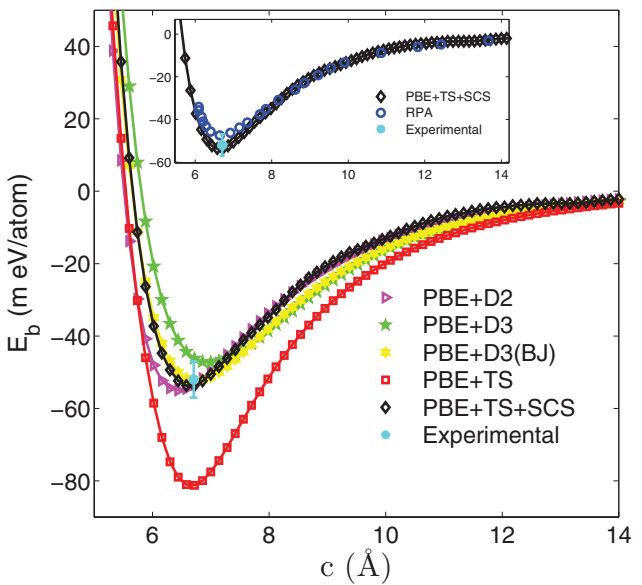
\includegraphics{_page_8_Figure_2.png}


\textbf{Figure 2.} Graphite interlayer binding energy as a function of the interlayer lattice parameter c. Shown are the Eb( ) c 's calculated with PBE + D2 (magenta open triangles), PBE + D3 (green solid stars), PBE + D3-BJ (yellow solid hexagons), PBE + TS (red open squares), and PBE + TS + SCS (black open diamonds), and the experimental binding energies (cyan filled circle). The solid lines represent the Chebyshev interpolation described in appendix A. The inset compares the PBE + TS + SCS (black open diamonds) and RPA (open blue circles) binding energies to the experimental data (cyan open circle).

The TS value for C33 is closer to the measured elastic constant than the TS + SCS result, just like the TS value for B0 is closer to the measured bulk modulus than the TS + SCS result. While it yields more accurate binding energies, screening degrades the TS estimate for the curvature of the potential-energy surface. The D3 and D3-BJ data in table 1 clearly show that the curvature of the interlayer binding energy critically depends on the damping function. We conclude that the development of more reliable damping functions may warrant better agreement with experimental data. Among the studied vdW corrections, the TS, TS + SCS, and D2, in that order, yield the best estimates for C33. We next compare the C333 coefficients from vdW corrections with the RPA result, 530 GPa [56]. This value is substantially larger than the −C333 resulting from the vdW corrections. The RPA tends to underestimate the binding energy at short distances, a trend that is expected to affect its derivatives in the vicinity of the equilibrium separation. Nonetheless, the resulting deviations are unlikely to account for the sizable discrepancies between the RPA and the vdW results in the −C333 column of table 1. D3, which includes long-range screening, yields the poorest agreement, but even the other corrections come to only third of the RPA value.

\subsubsection{\textit{III.F. Band structure analysis}}

As explained in section II, for given atomic configuration, i.e. for fixed geometry, the vdW corrections simply shift the DFT-PBE total energy. At fixed lattice and atomic parameters,


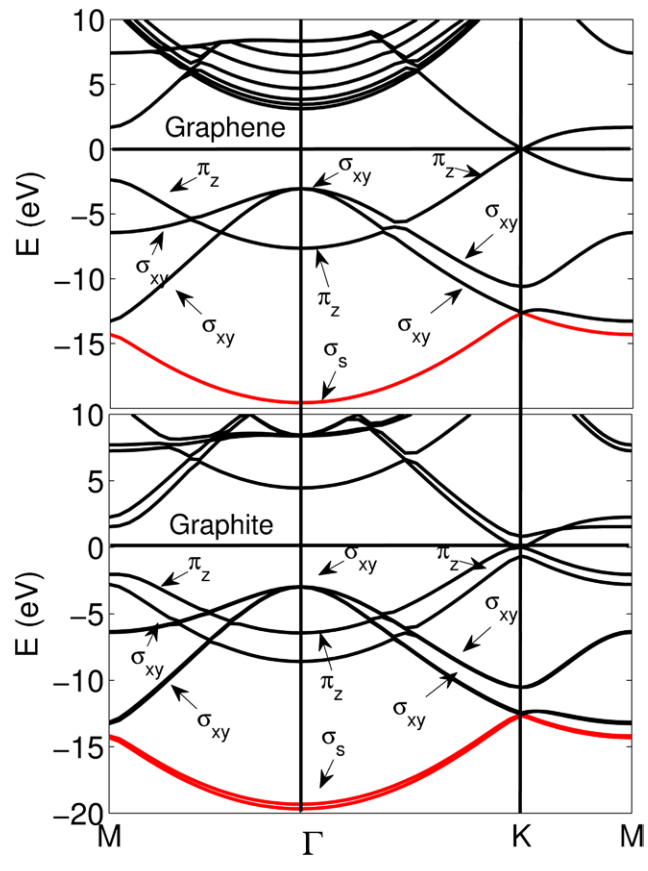
\includegraphics{_page_8_Figure_7.png}


\textbf{Figure 3.} The band structures of graphene (a = 2.46 A˚ 0 ), calculated with the standard PBE functional, and bulk graphite (a = 2.46 A˚ 0 , c = 20.1 A˚ ), calculated with the TS + SCS scheme. The symmetries of the most important bands (σs, σxy, πz) are indicated.

the electron density and the band structure are independent of the Etot vdW. The corrections nevertheless change the equilibrium lattice parameters and hence indirectly affect the band structure. Figure 3 shows the PBE band structures for two lattice structures, namely the equilibrium graphite PBE + TS + SCS structure (a = 2.466 A˚ 0 , c = 20.1 A˚ ) and a graphene layer (a = 2.466 A˚ 0 ). The two band structures are very similar, except for differences due to interlayer interations. For example, the πz- and σs-bands are degenerate in graphene, but the same bands are split at the Γ-point in graphite, due to the interlayer interactions. The very small σs splitting depends on intralayer states. By contrast, the πz-band splitting is substantial (for the PBE + TS + SCS structure, ∆πz = 2.14 eV) as one would expect, since the π bands come from the pz states perpendicular to the honeycomb layers. We therefore discuss the results for the πz band in more detail.

We have calculated ∆πz as a function of the interlayer distance for the PBE functional. The solid line in figure 4 depicts the results. Also shown in the figure are the splittings ∆πz for the D2, D3, D3-BJ, TS, and TS + SCS structures and the available experimental data [70, 71]. The ∆πz resulting from the vdW-corrected calculations vary from 0.56eV at c = 8.32 A˚ to 2.38 eV at c = 6.45 A˚ ). Experimentally, at c = c0, ∆πz = 2.4 eV [70] or ∆πz = 2.6 eV [71].


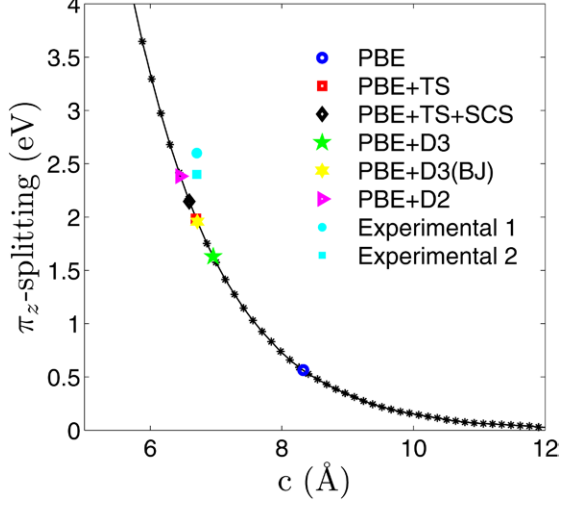
\includegraphics{_page_9_Figure_1.png}


\textbf{Figure 4.} Layer-separation dependence of the πz-level splitting. The symbols are the results of the indicated computational methods at the equilibrium separations. The solid curve represents the PBE splitting as a function of c. The cyan filled circle and square show the experimental splittings at the experimental equilibrium separation.

The solid curve in figure 4 is very well reproduced by the fit ∆πz = − A B 1 1 exp( ) c with A1 = 436.74eV and = − B 0.76 A˚ 1 1 . This decay of the πz-band splitting mirrors the exponential reduction of the overlap between carbon orbitals in neighboring layers as the layer separation grows. The blue open circle representing the PBE result in figure 4 lies far from the experimental points, because the functional manifestly overestimates the interlayer separation. The vdW corrections improve the agreement. For the PBE + TS + SCS vdW correction, in particular, the relative error is 10.6\%. Nonetheless, even at the experimental distance c = 6.707 A˚ 0 , the solid curve lies significantly below the experimental splittings. The plot in figure 4 therefore shows that the vdW corrections are insufficient to determine ∆πz with less than 10\% deviation. The XC functional will have to be improved before more accurate description of the graphite band structure can be achieved.

\subsubsection{\textit{III.G. PBE0 calculation}}

For the experimental lattices constants c = 6.707 A˚ 0 and a = 2.462 A˚ 0 , the hybrid functional PBE0 yields the band splitting ∆πz = 2.20 eV. Since ∆πz at fixed lattice parameters is insensitive to the vdW corrections, we can see that this computationally more demanding functional offers no significant improvement upon the PBE estimate for the band splitting.

\subsubsection{IV. \textbf{Conclusion}}

We have studied the properties of graphite in the DFT-PBE framework with several vdW corrections, namely D2, D3, D3-BJ, TS, and TS + SCS. We have computed several properties for which experimental results are available: the equilibrium lattice parameters a0 and c0, cohesive energy Ecoh, interlayer binding energy Eb, bulk modulus B0, curvature of the interlayer binding energy C33, C333, and πz-splitting at the Γ-point. The TS + SCS correction, which self-consistently accounts for dynamic screening, yields results in fair to good agreement with the experimental data.

Nonetheless, even the TS + SCS correction leaves room for improvement, a conclusion that is highlighted by the 30\% relative error in the calculated elastic constant C33 and the striking disagreement with the RPA result for C333. The other studied vdW corrections (D2, D3, D3-BJ, and TS) yield relatively large disagreement with the experimental data for one (D3-BJ), or two (D2, D3, TS) of the selected properties. In practical terms, should convergence problems or computational-cost considerations bar self-consistent approaches, our results would recommend the D3-BJ correction. We have also shown that the damping function controls the accuracy of the results for the elastic constant C33.

\subsubsection{\textbf{Acknowledgments}}

We are grateful to the São Paulo Science Foundation (FAPESP) and the Brazilian National Program of PosDocs (PNPD/CAPES) for the financial support and the São Carlos Informatic Center of São Paulo University for the infrastructural support of our cluster.

\section{\textbf{Appendix A. Numerical computation of the elastic constants} C\textbf{33 and} C333}

As equations (16) and (17) show, the elastic constant C33 and C333 can be computed from the interlayer-separation dependence of the binding energy Eb. In practice, the binding energies are only known at a set of discrete separations cj (j J = … 1, 2, , ), and a numerical procedure is required to compute the second and third derivatives d E d/ c 2 b 2 and d E d/ c 3 b 3 at the equilibrium separation c0. Given that the c dependences contain small oscillations superimposed on the broad minima—the oscillations are difficult to discern at the scale of the figure, but become visible under magnification—, to compute the derivatives, spectral methods are superior to finite-difference methods. Spectral methods are more accurate because they rely on information drawn from a relatively large number of data points, while finite-difference methods extract the derivatives from much smaller data sets. Were the binding-energy curves periodic, Fourier series would be the most recommended approach. Since the curves are not periodic, projection upon Chebyshev polynomials is preferable.

To optimize the computation of the curvature and its derivative at the equilibrium position, we first have to choose the interval defining the projection. To this end, given a sequence of symbols defining a curve in figure 2, we choose the interval ranging from the smallest \textit{cj j} = c min such that Eb < 0 to cJ. We then linearly scale the c axis so that the interval \textit{cj J} min ⩽ ⩽c c maps onto the interval −1 1 ⩽ ⩽x . Next, to choose the (nonuniform) mesh that will define the projection, we pick the number N of mesh points so that each mesh point is (approximately) one of the roots of the Nth order Chebyshev polynomial TN(x). More specifically, N is the largest integer such that no two roots of TN(x) lie between two successive points along the uniform mesh of the cj in figure 2.

Once the mesh is defined, we write the binding-energy curve as a N − 1 order Chebyshev series

$E_{b}(x)=\sum_{n=0}^{N-1}c_{n}T_{n}(x)$, (A.1)

i.e. project Eb( ) x upon the basis of the Chebyshev polynomials Tn(x) (n = …0, , 1 N − ). Since each derivative ( ) ( ) d / T x dx n m m (m = … 1, 2, ) is a linear combination of the n − m first Chebyshev polynomials, it is then a simple matter to numerically compute d / E x b( ) dx, d / E x( ) dx 2 b 2 , and d / E x( ) dx 3 b 3 . The equilibrium parameter c0 is then determined as the c value linearly mapped onto the root of d / E x b( ) dx, and the derivatives [d / E x( ) dx ] b c 2 2 0 and [d / E x( ) dx ] b c 3 3 0 needed to compute C33 and C333 from equations (16) and (17) can be easily evaluated.

\subsubsection{\textbf{References}}
\begin{itemize}
\item 
[1] Andreoni W (ed) 2000 \textit{The Physics of Fullerene-Based and Fullerene-Related Materials} (Berlin: Springer)

\item 
[2] Geim A K and Novoselov K S 2007 \textit{Nat. Mater.} 6 183

\item 
[3] Shaji S and Radhakrishnan V 2003 \textit{J. Mater. Process. Technol.} 141 51

\item 
[4] Novoselov K S, Geim A K, Morozov S V, Jiang D, Zhang Y, Dubonos S V, Gregorieva I V and Firsov A A 2004 \textit{Science} 306 666

\item 
[5] Castro A H, Guinea F, Peres K N M R and Geim A K 2009 \textit{Rev. Mod. Phys.} 81 109

\item 
[6] Ruiyi L, Juanjuana Z, Zhouping W, Zaijuna L, Junkanga L, Zhiguoa G and Guangli W 2015 \textit{Sensors Actuators} B 208 421

\item 
[7] Gobre V V and Tkatchenko A 2013 \textit{Nat. Commun.} 4 1

\item 
[8] Magda G Z, Jin X, Hagymási I, Vancsó P, Osváth Z, Nemes-Incze P, Hwang C, Biró L P and Tapasztó L 2014 \textit{Nature} 514 608

\item 
[9] Bernal J D 1924 \textit{Proc. R. Soc. Lond.} 106 749

\item 
[10] Haering R R 1958 \textit{Can. J. Phys.} 36 352

\item 
[11] Cong C, Yu T, Sato K, Shang J, Saito R, Dresselhaus G F and Dresselhaus M S 2011 \textit{ACS Nano} 5 8760

\item 
[12] Kleis J, Schrüder E and Hyldgaard P 2008 \textit{Phys. Rev.} B 77 205422

\item 
[13] Churkin Y V, Fedortsov A B, Klimchitskaya G L and Yurova V A 2010 \textit{Phys. Rev.} B 82 165433

\item 
[14] Girifalco L A and Lad R A 1956 \textit{J. Chem. Phys.} 25 693

\item 
[15] Benedict L X, Chopra N G, Cohen M L, Zettl A, Louie S G and Crespi V H 1998 \textit{Chem. Phys. Lett.} 286 490

\item 
[16] Zacharia R, Ulbricht H and Hertel T 2004 \textit{Phys. Rev.} B 69 155406

\item 
[17] Liu Z, Liu J Z, Cheng Y, Li Z, Wang L and Zheng Q 2012 \textit{Phys. Rev.} B 85 205418

\item 
[18] Hohenberg P and Kohn W 1964 \textit{Phys. Rev.} 136 B864

\item 
[19] Kohn W and Sham L J 1965 \textit{Phys. Rev.} 140 A1133

\item 
[20] Perdew J P, Burke K and Ernzerhof M 1996 \textit{Phys. Rev. Lett.} 77 3865

\item 
[21] Perdew J P, Chevary J A, Vosko S H, Jackson K A, Pederson M R, Singh D J and Fiolhais C 1992 \textit{Phys. Rev.} B 46 6671

\item 
[22] Silva J L F D and Stampfl C 2007 \textit{Phys. Rev.} B 76 085301

\item 
[23] Kristyán S and Pulay P 1994 \textit{Chem. Phys. Lett.} 229 175

\item 
[24] Tkatchenko A and von Lilienfeld O A 2008 \textit{Phys. Rev.} B 78 045116

\item 
[25] Stoll H 1992 \textit{J. Chem. Phys.} 97 8449

\item 
[26] Foulkes W M C, Mitas L, Needs R and Rajagopal G 2001 \textit{Rev. Mod. Phys.} 73 33

\item 
[27] Sorella S, Casula M and Rocca D 2007 \textit{J. Chem. Phys.} 127 014105

\item 
[28] Furche F 2001 \textit{Phys. Rev.} B 64 195120

\item 
[29] Lèbegue S, Harl J, Gould T, Ángyán J G, Kresse G and Dobson J F 2010 \textit{Phys. Rev. Lett.} 105 196401

\item 
[30] Spanu L, Sorella S and Galli G 2009 \textit{Phys. Rev. Lett.} 103 196401

\item 
[31] Barone V, Casarin M, Forrer D, Pavone M, Sambi M and Vittadini A 2009 \textit{J. Comput. Chem.} 30 934

\item 
[32] Grimme S, Antony J, Ehrlich S and Krieg H 2010 \textit{J. Chem. Phys.} 132 154104

\item 
[33] Björkman T, Gulans A, Krasheninnikov A V and Nieminen R M 2012 \textit{J. Phys.: Condens. Matter} 24 424218

\item 
[34] Björkman T 2014 \textit{J. Chem. Phys.} 141 074708

\item 
[35] Tkatchenko A and Scheffler M 2009 \textit{Phys. Rev. Lett.} 102 073005

\item 
[36] Tkatchenko A, DiStasio R A, Car R and Scheffler M 2012 \textit{Phys. Rev. Lett.} 108 236402

\item 
[37] Grimme S 2006 \textit{J. Comput. Chem.} 27 1787

\item 
[38] Blum V, Gehrke R, Hanke F, Havu P, Havu V, Ren X, Reuter K and Scheffler M 2009 \textit{Comput. Phys. Commun.} 180 2175

\item 
[39] Kresse G and Hafner J 1993 \textit{Phys. Rev.} B 48 13115

\item 
[40] Kresse G and Furthmüller J 1996 \textit{Phys. Rev.} B 54 11169

\item 
[41] Bucko T, Lèbegue S, Hafner J and Ángyán J G 2013 \textit{Phys. Rev.} B 87 064110

\item 
[42] Bucko T, Hafner J, Lèbegue S and Ángyán J G 2010 \textit{J. Phys. Chem.} A 114 11814

\item 
[43] Bucko T, Lèbegue S, Hafner J and Ángyán J G 2013 \textit{J. Chem. Theory Comput.} 9 4293

\item 
[44] Axilrod B M and Teller E 1943 \textit{J. Chem. Phys.} 11 299

\item 
[45] Ambrosetti A, Reilly A M, DiStasio R A and Tkatchenko A 2014 \textit{J. Chem. Phys.} 140 18A508

\item 
[46] Adamo C and Barone V 1999 \textit{J. Chem. Phys.} 110 6158

\item 
[47] Casimir H B G and Polder D 1948 \textit{Phys. Rev.} B 73 360

\item 
[48] Tkatchenko A, Ambrosetti A and DiStasio R A 2013 \textit{J. Chem. Phys.} 138 074106

\item 
[49] Silvestrelli P L and Ambrosetti A 2014 \textit{J. Chem. Phys.} 140 124107

\item 
[50] Grimme S, Ehrlich S and Goerigk L 2011 \textit{J. Comput. Chem.} 32 1456

\item 
[51] Blöchl P E 1994 \textit{Phys. Rev.} B 50 17953

\item 
[52] Kresse G and Joubert D 1999 \textit{Phys. Rev.} B 59 1758

\item 
[53] Zhao Y X and Spain I L 1989 \textit{Phys. Rev.} B 40 993

\item 
[54] Hanfland M, Beister H and Syassen K 1989 \textit{Phys. Rev.} B 39 12598

\item 
[55] Bosak A, Krisch M, Mohr M, Maultzsch J and Thomsen C 2007 \textit{Phys. Rev.} B 75 153408

\item 
[56] Gould T, Lebegue S and Dobson J F 2013 \textit{J. Phys.: Condens. Matter} 25 445010

\item 
[57] Kittel C 1996 \textit{Introduction to Solid State Physics} 7th edn (New York: Wiley)

\item 
[58] Haas P, Tran F and Blaha P 2009 \textit{Phys. Rev.} B 79 085104

\item 
[59] Rydberg H, Dion M, Jacobson N, Schröder E, Hyldgaard P, Simak S I, Langreth D C and Lundqvist B I 2003 \textit{Phys. Rev. Lett.} 91 126402

\item 
[60] Blakslee O L 1970 \textit{J. Appl. Phys.} 41 3373

\item 
[61] Yin M T and Cohen M L 1984 \textit{Phys. Rev.} B 29 6996

\item 
[62] Ernzerhof M and Scuseria G E 1999 \textit{J. Chem. Phys.} 110 5029

\item 
[63] Fuchs M, Da Silva J L F, Stampfl C, Neugebauer J and Scheffler M 2002 \textit{Phys. Rev.} B 65 245212

\item 
[64] Da Silva J L F, Stampfl C and Scheffler M 2006 \textit{Surf. Sci.} 600 703

\item 
[65] Olsen T and Thygesen K S 2013 \textit{Phys. Rev.} B 87 075111

\item 
[66] Shin H, Kang S, Koo J, Lee H, Kim J and Kwon Y 2014 J. \textit{Chem. Phys.} 140 114702

\item 
[67] Birch F 1947 \textit{Phys. Rev.} 71 809

\item 
[68] Gauster W B and Fritz I J 1974 \textit{J. Appl. Phys.} 45 3309

\item 
[69] Jansen H J F and Freeman A J 1987 \textit{Phys. Rev.} B 35 8207

\end{itemize}

View publication stats
\begin{itemize}
\item 
[70] Law A R, Barry J J and Hughes H P 1983 \textit{Phys. Rev.} B 28 5332

\item 
[71] Zhou S Y, Gweon G-H, Spataru C D, Graf J, Lee D-H, Louie S G and Lanzara A 2005 \textit{Phys. Rev.} B 71 161403

\end{itemize}
\end{document}
